%%%%%%%%%%%%%%%%%%%%%%%%%%%%%%%%%%%%%%%%%
% Journal Article
% LaTeX Template
% Version 1.3 (9/9/13)
%
% This template has been downloaded from:
% http://www.LaTeXTemplates.com
%
% Original author:
% Frits Wenneker (http://www.howtotex.com)
%
% License:
% CC BY-NC-SA 3.0 (http://creativecommons.org/licenses/by-nc-sa/3.0/)
%
%%%%%%%%%%%%%%%%%%%%%%%%%%%%%%%%%%%%%%%%%

%----------------------------------------------------------------------------------------
%	PACKAGES AND OTHER DOCUMENT CONFIGURATIONS
%----------------------------------------------------------------------------------------

\documentclass[twoside]{article}

\usepackage{lipsum} % Package to generate dummy text throughout this template
\usepackage{graphicx}
\usepackage[sc]{mathpazo} % Use the Palatino font
\usepackage[T1]{fontenc} % Use 8-bit encoding that has 256 glyphs
\linespread{1.05} % Line spacing - Palatino needs more space between lines
\usepackage{microtype} % Slightly tweak font spacing for aesthetics

\usepackage[hmarginratio=1:1,top=32mm,columnsep=20pt]{geometry} % Document margins
\usepackage{multicol} % Used for the two-column layout of the document
\usepackage[hang, small,labelfont=bf,up,textfont=it,up]{caption} % Custom captions under/above floats in tables or figures
\usepackage{booktabs} % Horizontal rules in tables
\usepackage{float} % Required for tables and figures in the multi-column environment - they need to be placed in specific locations with the [H] (e.g. \begin{table}[H])
\usepackage{hyperref} % For hyperlinks in the PDF

\usepackage{lettrine} % The lettrine is the first enlarged letter at the beginning of the text
\usepackage{paralist} % Used for the compactitem environment which makes bullet points with less space between them

\usepackage{abstract} % Allows abstract customization
\renewcommand{\abstractnamefont}{\normalfont\bfseries} % Set the "Abstract" text to bold
\renewcommand{\abstracttextfont}{\normalfont\small\itshape} % Set the abstract itself to small italic text

\usepackage{titlesec} % Allows customization of titles
\renewcommand\thesection{\Roman{section}} % Roman numerals for the sections
\renewcommand\thesubsection{\Roman{subsection}} % Roman numerals for subsections
\titleformat{\section}[block]{\large\scshape\centering}{\thesection.}{1em}{} % Change the look of the section titles
\titleformat{\subsection}[block]{\large}{\thesubsection.}{1em}{} % Change the look of the section titles

\usepackage{fancyhdr} % Headers and footers
\pagestyle{fancy} % All pages have headers and footers
\fancyhead{} % Blank out the default header
\fancyfoot{} % Blank out the default footer
\fancyhead[C]{} % Custom header text
\fancyfoot[RO,LE]{\thepage} % Custom footer text

%----------------------------------------------------------------------------------------
%	TITLE SECTION
%----------------------------------------------------------------------------------------

\title{\vspace{-15mm}\fontsize{24pt}{10pt}\selectfont\textbf{Report on Bubble Blast Game}} % Article title

\author{
\large
\textsc{Prakhar Asthana}\thanks{Entry No:2011cs1027, B.tech 3rd Year, Computer Science and Engineering}\\[2mm] % Your name
\normalsize Indian Institute of Technology Ropar \\ % Your institution
\normalsize \href{mailto:prakharas@iitrpr.ac.in}{prakharas@iitrpr.ac.in} % Your email address
%%\vspace{1mm}
\date{25/12/2013}
}


%----------------------------------------------------------------------------------------

\begin{document}

\maketitle % Insert title

\thispagestyle{fancy} % All pages have headers and footers

%----------------------------------------------------------------------------------------
%	ABSTRACT
%----------------------------------------------------------------------------------------

\begin{abstract}

\noindent This report is about a game which goes by name \textit{BubbleBlast}. The report presents and discusses the empirical data of the vaious approaches to solve this game.  % Dummy abstract text

\end{abstract}

%----------------------------------------------------------------------------------------
%	ARTICLE CONTENTS
%----------------------------------------------------------------------------------------

\begin{multicols}{2} % Two-column layout throughout the main article text

\section{Introduction}

\lettrine[nindent=0em,lines=3]{\textit{B}} {ubbleblast} is also known as \textit{SameGame} and \textit{Clickomania}. It was first invented by \textit{Kuniaki Moribe} under the name \textit{ChainShot!} in 1985. It was created again under name \textit{SameGame} by \textit{Eiji Fukumoto} in 1992$^{[2]}$. In this report, author discusses the various approaches to solve this game.% Dummy text

%------------------------------------------------

\section{Description of Game}

Initial Game setup and rules are as under 
\begin{enumerate}
\item This game is played on a rectangular grid of size $mxn$ where $m$ denotes number of horizontal rows and $n$ denotes number of vertical coloumns. 
\item Initialy each cell of grid has a \textit{bubble} of some \textit{color}.
\item \textit{Color} of a \textit{bubble} is denoted by an integer in interval [$1,k$], $1<=k<=m*n$. Here, different integer value denotes different \textit{color} and vice-versa . $k$ is maximum number of $colors$ possible. 
\item We define a position ($i,j$) on grid as cell at intersection of $i^{th}$ row and $j^{th}$ coloumn. $0<=i<m , 0<=j<n$.
\item A position ($i,j$) is called $empty$ if the cell present at that position does not have a bubble. Color of such a cell is denoted by integer value 0. Initially all the cells are $non-empty$. 
\item If all the cells in a vertical coloumn are empty it is called an $empty$ $ coloumn$.
\item A $block$ is defined as a \textbf{maximal} set of \textbf{2 or more} bubbles of \textbf{same} color such that it is possible to visit any bubble to any other bubble in block following 4- neighbourhood connectvity.
\item $Size$ of a block is defined as no. of bubbles in that block.
\item A bubble is in  $singleton$ state when it does not belong to any block. 
\item Deleting the block means removing all the bubbles belonging to that block from the grid.
\item A $blast$ means deleting a block from the grid and after that making changes in the grid following rules of $vertical$ and $horizontal$ $shift$ \textbf{inorder} defined as under:
\begin{enumerate}
	\item Vertical Shift : When a bubble is deleted from the grid, all the bubbles above that bubble are shifted down and the topmost position is padded with an empty cell.
	\item Horizontal Shift : After performing $Vertical$ $Shift$, if a coloumn becomes empty then the all the coloumns to the left of it are shifted right and the leftmost coloumn is padded with an empty coloumn. 
\end{enumerate}
\item Each blast generates a $score$ which is defined as square of the size of the block deleted in that move.
\item Game ends when all the bubbles are blasted or there are no further blocks possible i.e. all remaining bubbles are in singleton state.
\end{enumerate}
\begin{center}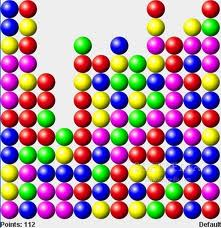
\includegraphics[width=4cm]{index.jpeg}\end{center}
Our aim is to blast the bubbles in a way to obtain maximum total score.

\section{Complexity}
\begin{enumerate}
\item It has been proven that the problem of determining that whether a given grid can be completely emptied or not is NP-complete$^{[3]}$. 
\item Further it is also proved the problem of finding the sequence of blasts which results in maximum total score \textbf{independent of its scoring function} is also NP-complete$^{[2]}$.
\end{enumerate}
Further in the report the author discusses various approaches that can be followed to tackle a given grid.
%------------------------------------------------
\section{Various Approaches}
\begin{enumerate}
\item Always pick a random non-empty non-singleton position and blast the bubble block at that position.
\item Always blast the \textbf{minimum} size block of the \textbf{least} frequent color if possible. Move to higher frequency colors inorder if all the bubble of less frequent colors are in singleton state or have already been blasted. This is known as \textit{TabuColorRandom} strategy$^{[2]}$. Any ties are broken arbitrarily.
\item Starting from least frequent color and moving to higher frequency colors inorder, pick the color with least frequency whose block is possible. If the color lies in bottom 1/3$^{rd}$ of color array sorted by their frequency then blast the maximum sized block of that color. Otherwise, blast the minimum sized block. Any ties are broken arbitrarily.
\item Always blast the \textbf{maximum} size block of the \textbf{least} frequent color if possible. Move to higher frequency colors inorder if all the bubble of less frequent colors are in singleton state or have already been blasted. Any ties are broken arbitrarily.
\item Always blast the \textbf{maximum} size block of the \textbf{most} frequent color if possible. Move to lower frequency colors inorder if all the bubble of more frequent colors are in singleton state or have already been blasted.Any ties are broken arbitrarily.
\end{enumerate}
\section{Results}
All the approaches were tested over various inputs of various sizes and colors. Then the mean and standard deviation were calculated as under
\begin{table}[H]
\caption{Mean and standard deviation of total score}
\centering
\begin{tabular}{llr}
\toprule
%\multicolumn{2}{c}{Name} \\
%\cmidrule(r){1-3}
Approach & Mean & Standard Deviation\\
\midrule
1 & 3554.235 & 359.254 \\
2 & 20719.598 & 5491.497\\
3 & 20348.544 & 5658.565\\
4 & 9276.280 & 5667.464\\
5 & 3637.266 & 302.88\\
\bottomrule
\end{tabular}
\end{table}
As clear from the emiprical data, approach \#2 and \#3 give almost similar results but they are stringingly better than all other approaches. Reason for this is that approach \# 2, \#3 (and \#5 too) tries to build up block size of most frequent color and other more frequent colors over time. This results in an increase in \textit{Average Block Size}(see next page). Since our
 score function is quadratic in nature, it resuls in great increase in score due to fact
\begin{equation}
\label{eq:emc}
(a+b)^{2} \geq a^{2} + b^{2} 
\end{equation}
Thus keeping big blocks intact and blasting them later is better than blasting the block in form of various chunks as it gives higher score.\\\\
Figures below show the performance of all the approaches on a 25X25 grid with varying no. of colors. As clear from the figure too approach \#2 and \#3 give best results among all.
%\begin{figure}[ht]
%\begin{center}
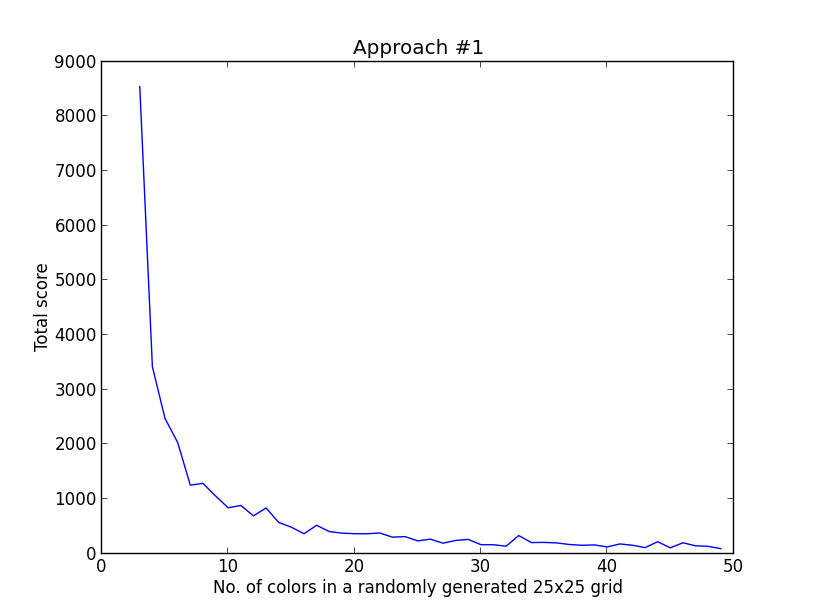
\includegraphics[width=8cm]{figure_3.png}
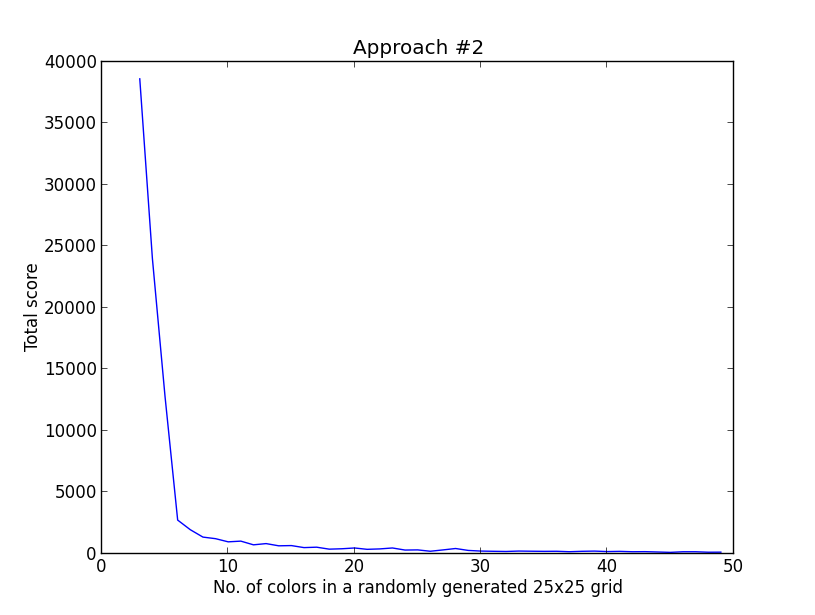
\includegraphics[width=8cm]{figure_2.png}
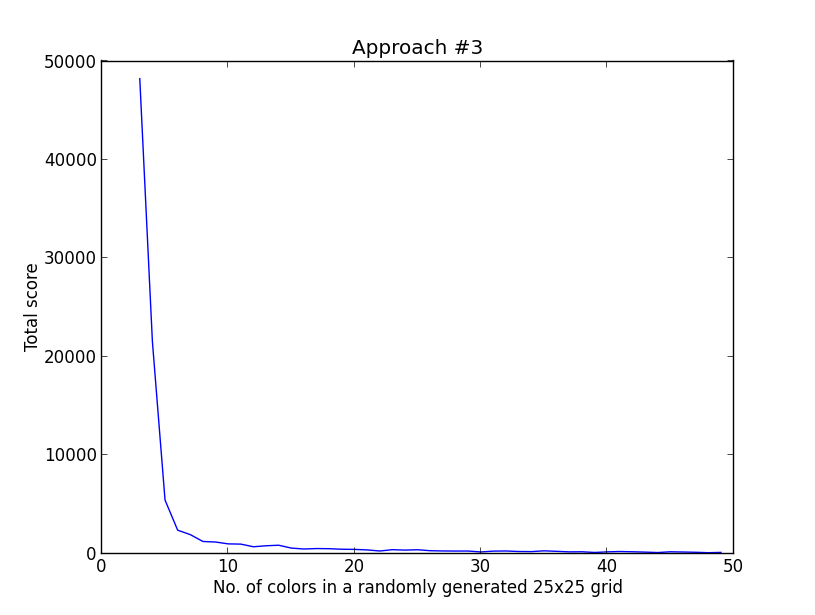
\includegraphics[width=8cm]{figure_1.png}
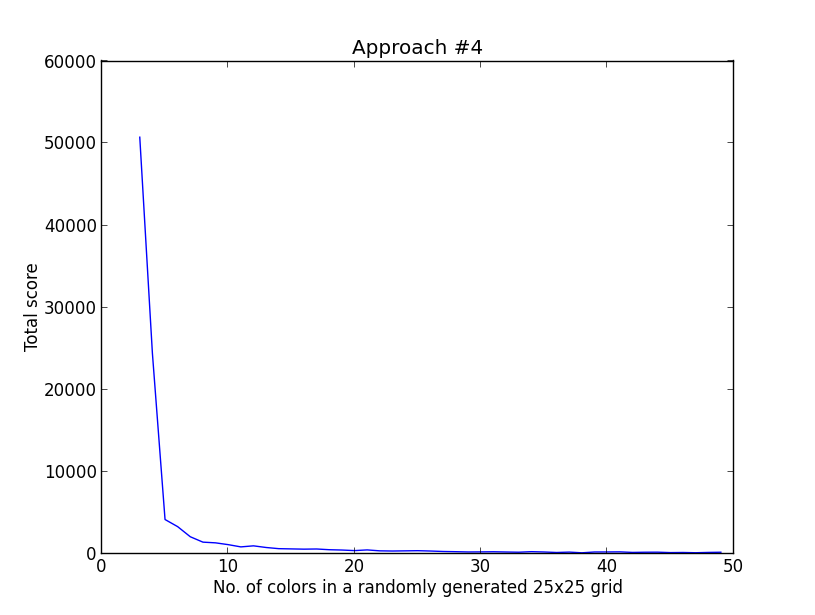
\includegraphics[width=8cm]{figure_4.png}
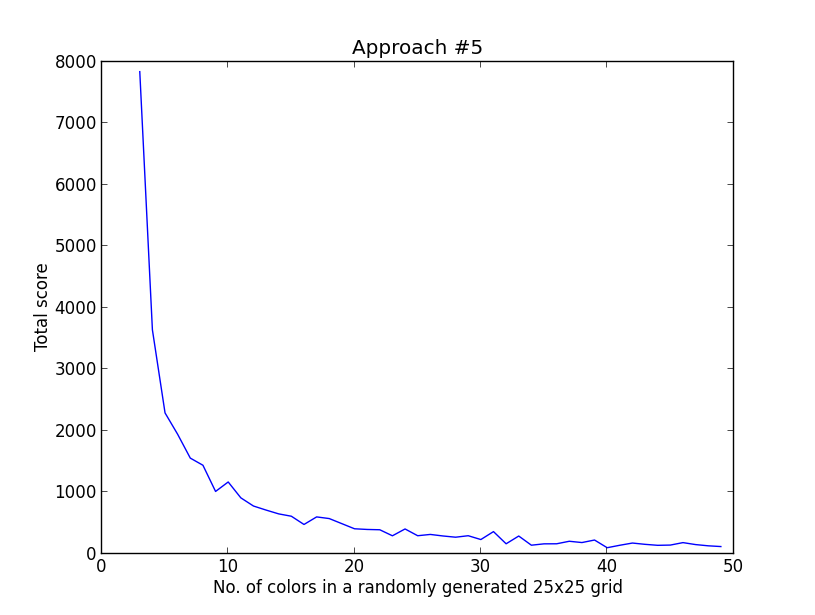
\includegraphics[width=8cm]{figure_5.png}
\emph{Score V number of colors ; Grid Size=25x25}\\
%\end{center}
%\end{figure}

Let us define \textit{Average Block Size} for a given grid as under
\begin{equation}
\label{eq:emc}
Average Block Size(ABS) =\sqrt{Total Score}
\end{equation}
Grids varying in size and number of colors were given as input to all the approaches and the mean and standard deviation of ABS is as under.

\begin{table}[H]
\caption{Mean and standard deviation of ABS}
\centering
\begin{tabular}{llr}
\toprule
%\multicolumn{2}{c}{Name} \\
%\cmidrule(r){1-3}
Approach & Mean& Standard Deviation \\
\midrule
1 & 61.414 & 3.304 \\
2 & 142.92 & 19.972\\
3 & 141.139 & 20.689\\
4 & 137.250 & 20.943\\
5 & 60.258 & 2.495\\
\bottomrule
\end{tabular}
\end{table}
As clear from the table, approach \#2 and \#3 have highest ABS and this is the reason they generate higher scores as compared to other approaches.\\ 
Figure below shows variation in ABS(y-axis) over 1000 different input grids for all 5 approaches
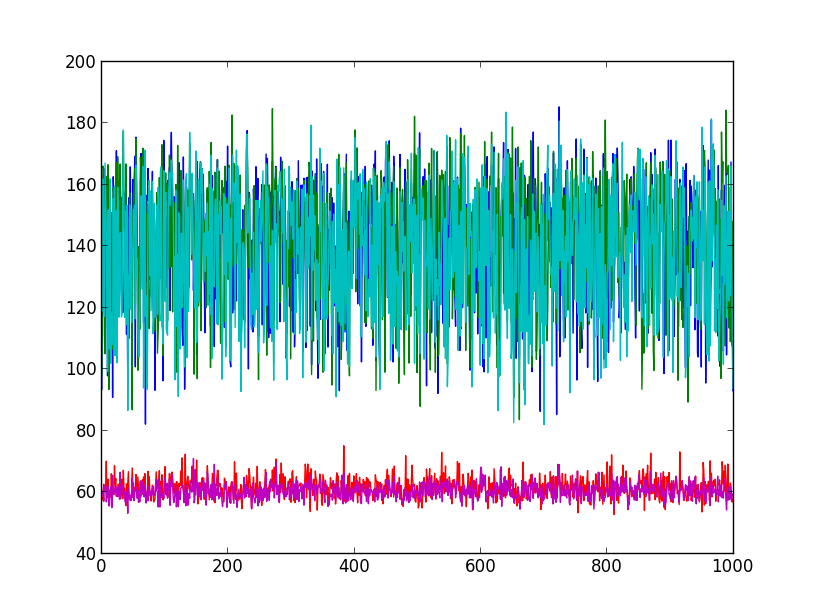
\includegraphics[width=9cm]{blocksize.png}
\footnotesize \emph{Red-Approach\#1; Green-Approach\#2; Blue-Approach\#3; SeaBlue-Approach\#4; Purple-Approach\#5 }\\
\normalsize
As clear form the figure above approach \#2, \#3 and \#4 has higher ABS values(100-160) while approach \#1 and \#5 have lower ABS values(60-70).


%------------------------------------------------

\section{Other Approaches}
Classical approach of solving puzzles are $A^{*}$ (removing the node from the front of the queue and storing all its children in the sorted order of the $key$ at the back of the queue till goal state is arrived) and $IDA^{*}$ (iterative depth- first version of $A^{*}$). Here $key$ is the value of evaluation function evaluated at that node.\\
But these methods fail work in our problem because it is not easy to find the evaluation function for Bubbleblast game.$^{[2]}$\\\\
Other techniques are Beam search and Depth Budgeted search$^{[1]}$. In Beam Search a $beam$ of best $B$ nodes is kept for each iteration. If in the process, a leaf node is reached it is checked whether it is better than the current best solution so far. Its complexity is $O(B*d)$ where $d$ is the maximum depth reached.\\
In Depth Budgeted search each node is allowed to explore the tree below it. Initial budget to each node is assigned through Banker's Algorithm$^{[1]}$. When the all the assigned budget gets used up, a greedy approach is followed to arrive at the solution.\\\\
So far the best known approach is \textbf{Monte Carlo with Roulette-Wheel Selection (MC-RWS)
}, which performs the Monte Carlo simulation on each node and chooses the one which is evaluated higher by evaluation function as defined in [1]
%----------------------------------------------------------------------------------------
%	REFERENCE LIST
%----------------------------------------------------------------------------------------
\section{References}
\begin{enumerate}
\item Takes, Frank W., and Walter A. Kosters. "Solving SameGame and its chessboard variant." Proceedings of the 21st Benelux Conference on Artificial Intelligence (BNAIC’09)(eds. T. Calders, K. Tuyls, and M. Pechenizkiy). 2009.
\item Schadd, Maarten PD, et al. "Addressing NP-complete puzzles with Monte-Carlo methods." Proceedings of the AISB 2008 Symposium on Logic and the Simulation of Interaction and Reasoning. Vol. 9. 2008.
\item Biedl, Therese C., et al. "The complexity of Clickomania." More games of no chance 42 (2002): 389.
\end{enumerate}
%----------------------------------------------------------------------------------------

\end{multicols}

\end{document}
